\justifying
\NSFCBodyText

\subsubsection{研究背景与意义}

对地观测数据的规模增长已经远远超过人工判读能力。在资源调查、国土监测、灾害应急等业务中，使用者真正需要的往往不是"某一景影像的编号"，而是"哪些影像里出现了某种地物组合与空间格局"。以自然语言直接检索遥感影像，因此成为把海量影像库转化为可用地理信息的一条关键途径：它不要求使用者预先掌握波段、传感器与产品级别等专业参数，也不受固定类别体系的限制，允许用一句自然描述表达带有空间关系的复合需求，例如"河流两侧分布着成排厂房"。 上述检索需求与描述覆盖不足之间的矛盾见图~\ref{fig:background}。

% F1: F01_研究背景与问题提出-v3.png
\begin{figure}[!htbp]
    \centering
    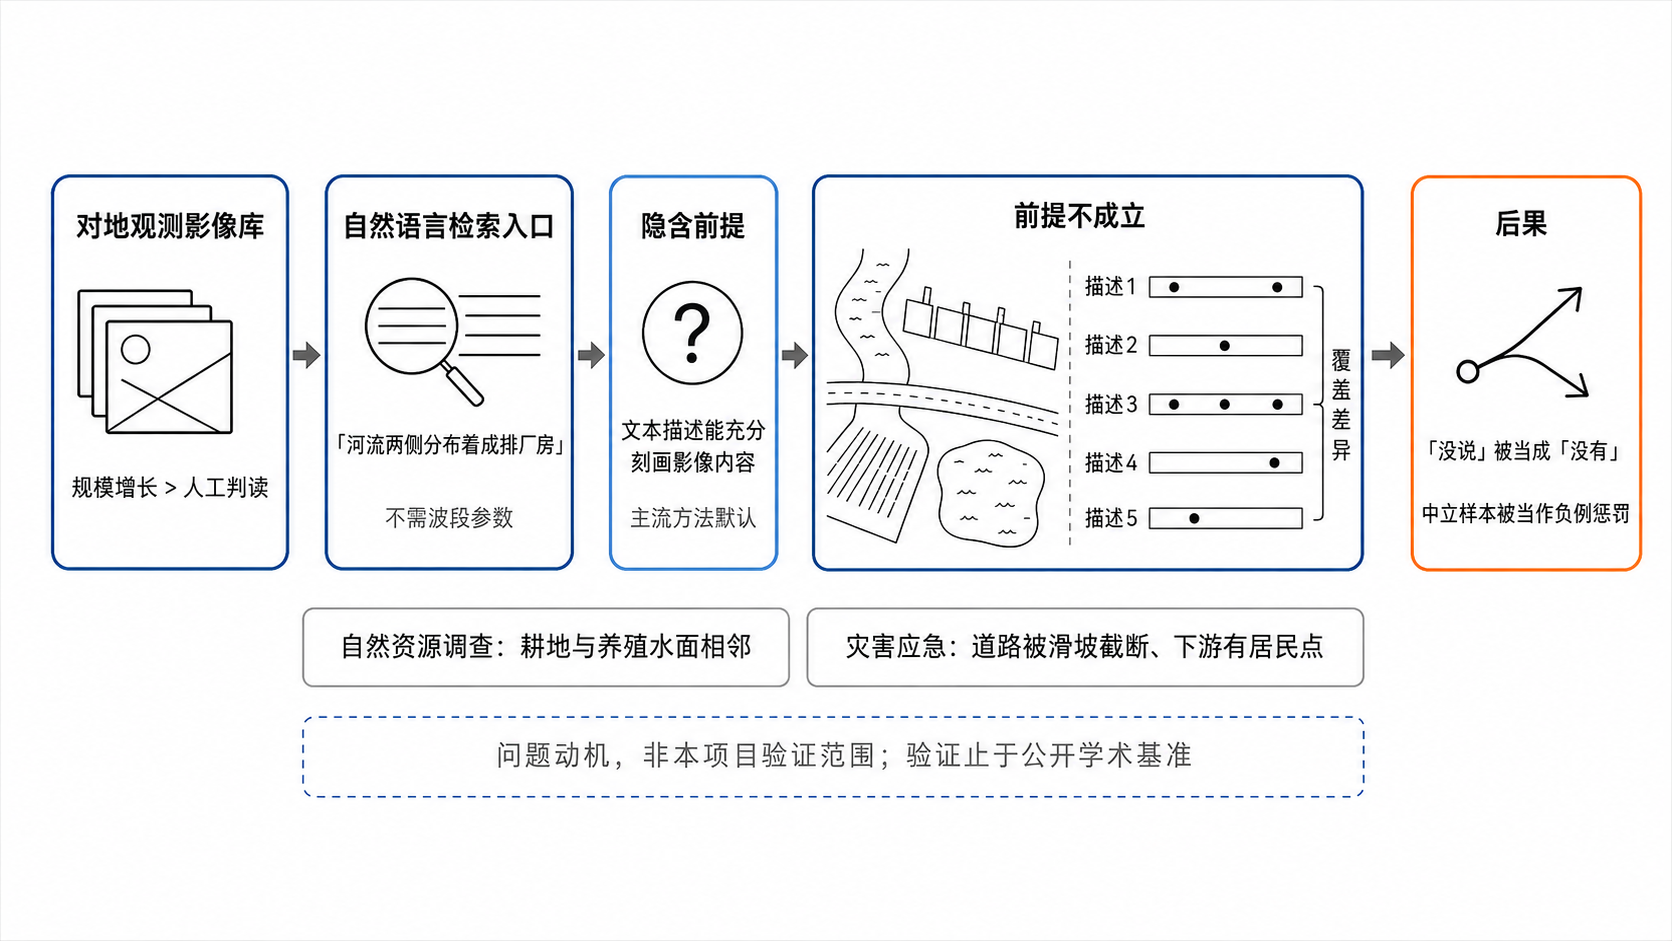
\includegraphics[width=\linewidth]{figures/F01_研究背景与问题提出-v3.png}
    \caption{研究背景与问题提出。业务场景用于说明研究动机，项目验证范围为公开学术基准。}
    \label{fig:background}
\end{figure}


围绕这一目标，遥感图文检索在近年形成了相对完整的研究体系。国内学者从多模态对齐的角度系统梳理了遥感领域时空对齐与语义对齐的发展脉络\cite{lishutao2025alignment}，并对遥感场景下图文跨模态理解的任务划分、公开数据与评价指标做了归纳\cite{zhengxiangtao2025crossmodal}；面向图文检索这一具体任务，视觉语言基础模型驱动下的研究进展也已被专门综述\cite{wuhui2026rsitr}。国际上，遥感视觉语言模型的能力边界与发展趋势同样得到系统评述\cite{li2024vlmrsmag}，并出现了对检索方法与数据基础演化的横向对比\cite{rsitrreview2025}。

然而，把自然语言当作检索入口，隐含着一个很少被正面处理的前提：\textbf{文本描述能够充分刻画影像内容}。这个前提在遥感场景中并不成立。一景遥感影像通常同时包含道路、建筑、水体、植被等多类地物及其复杂空间格局，而一条人工描述往往只覆盖其中一部分。公开基准的构建方式本身就说明了这一点：RSICD 为每幅影像配置 5 条描述\cite{lu2018rsicd}，RSITMD 进一步强调描述的细粒度与低冗余、每图配 5 条并附关键词\cite{yuan2022amfmn}——如果单条描述足以覆盖影像内容，就不需要多条互补的描述。

描述的不完备带来一个直接后果：当模型看到"影像中有而文本未提及"的内容时，无法判断这究竟意味着"描述没写到"还是"两者确实不一致"。在对比学习框架下，这种无法判断往往被默认按后者处理，从而把大量本应中立的样本当作负例来惩罚。\textbf{如何让模型在描述不完备的条件下正确使用地理实体关系，而不是把"没说"误当成"没有"，是本项目要回答的问题。} 这一问题对遥感尤为关键：地物之间的空间关系（相邻、包含、方位、距离）正是使用者最常用来表达检索意图的语义，也恰恰是最容易在描述中被省略的部分。 图~\ref{fig:three-state}示意描述覆盖差异导致的三态歧义及其监督处理方式。

% F2: F02_三态歧义.png
\begin{figure}[!htbp]
    \centering
    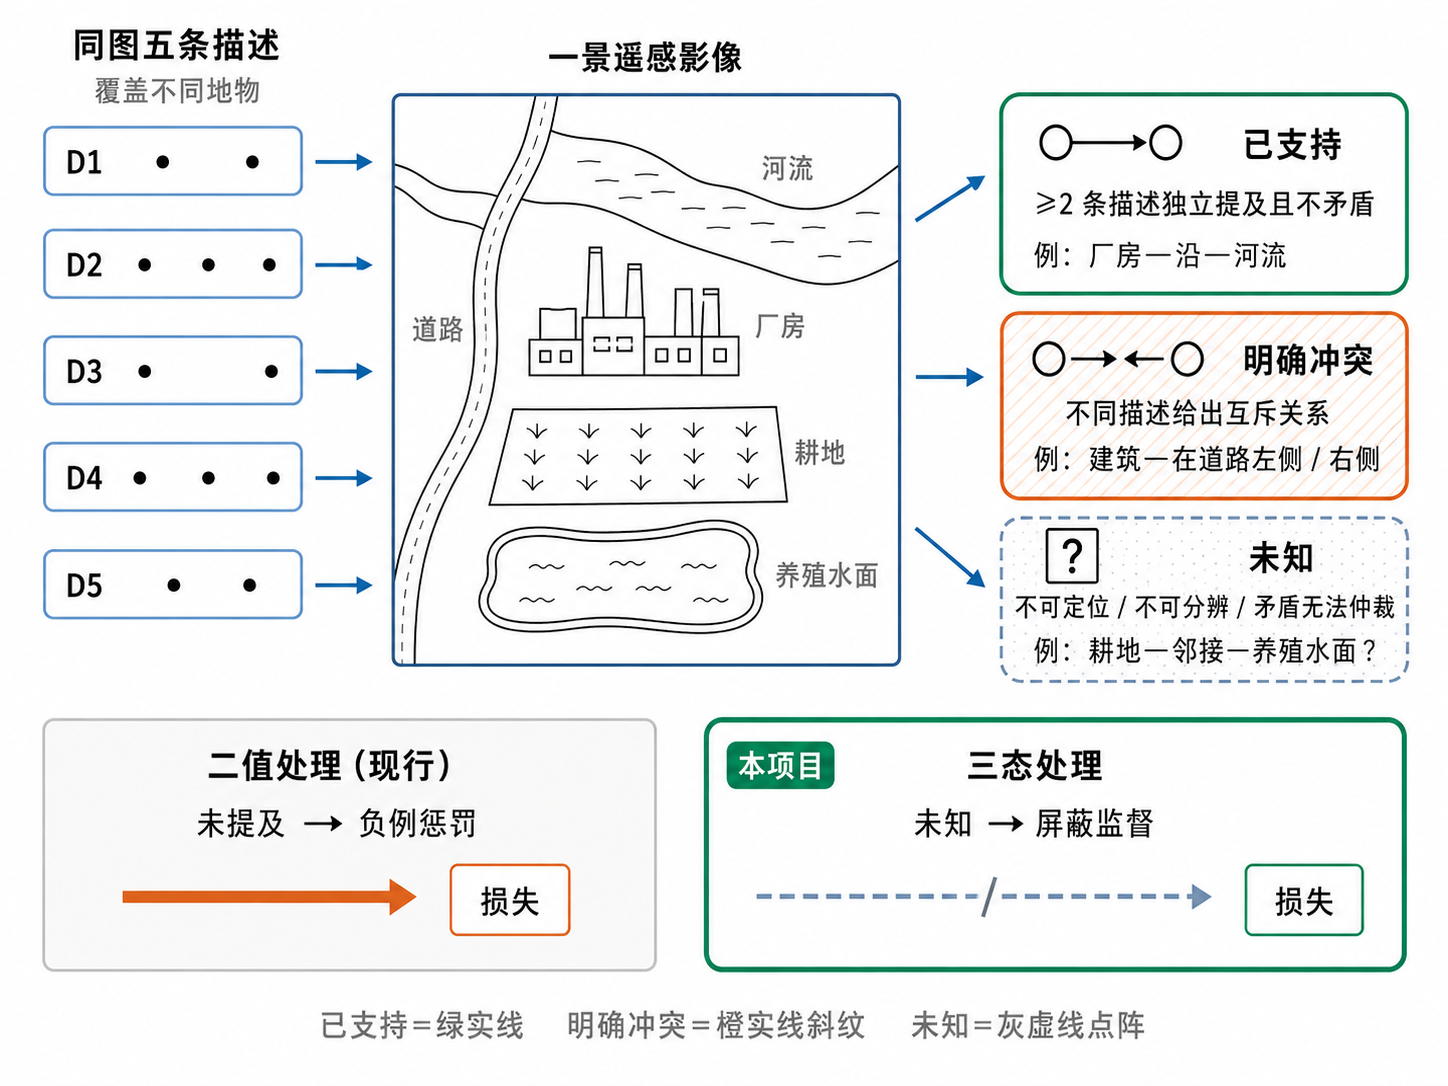
\includegraphics[width=0.90\linewidth]{figures/F02_三态歧义.png}
    \caption{描述不完备导致的三态歧义。未提及与明确冲突分开判定；未知关系不参与监督。}
    \label{fig:three-state}
\end{figure}


这一问题的现实分量可以从典型业务场景看出。在自然资源调查中，作业人员需要从历史影像库中找出"耕地与养殖水面相邻"的地块以核查用途变化；在灾害应急中，需要快速定位"道路被滑坡体截断、下游有居民点"的区域。这些需求的共同点是：检索意图由\textbf{地物及其空间关系}共同定义，而非单个地物类别。也正因如此，检索系统对关系的处理方式直接决定其可用性——把"文本没提到水体"理解为"影像里不应有水体"，会让大量本应召回的影像被排除；反过来，若对关系一概不作约束，"建筑在道路左侧"与"建筑在道路右侧"就无法区分。

这里需要把话说清楚：上述场景说明的是\textbf{问题为什么值得研究}，不是本项目的验证范围。业务型数据涉及权属、精度与保密要求，本项目不具备获取条件，也不承诺业务落地。本项目的验证止于公开学术基准（RSITMD、RSICD）及在其上构建的关系挑战评测；从基准结论到业务应用之间还隔着数据域差异与作业规范适配，属后续工作。把方法问题在公开基准上研究清楚，是通向业务可用的前提，但不等同于业务可用。

本项目的科学价值在于澄清跨模态匹配中一个被长期默认接受的建模前提，并把"关系证据是否可判定"这一变量的表示方式、学习方式与验证方式一并给出。这一前提的修正不限于遥感图文检索：凡是监督信号由"配对与否"隐式定义、而描述又天然不完备的跨模态任务，都面临同类困境。应用价值则体现在可解释性上——业务用户需要知道一景影像被排除，究竟是因为它不符合要求，还是因为描述里恰好没写。对承担核查责任的自然资源与测绘业务而言，这一区分直接决定检索结果能否被采信。

\subsubsection{国内外研究现状及发展动态分析}

\subsubsubsection{任务基准与评测口径}

遥感图文检索的基准体系以 RSICD\cite{lu2018rsicd} 与 RSITMD\cite{yuan2022amfmn} 为核心，评测普遍采用双向 R@1/R@5/R@10 及六项均值 mR。近年出现了规模更大、语义更丰富的数据资源：SkyScript 将影像与开放地理数据的语义相连接\cite{wang2024skyscript}，RS5M 构建了大规模遥感图文数据并训练了相应模型\cite{zhang2024rs5m}，LuoJiaHOG 则从层次化、地理感知的角度组织图像描述\cite{zhao2025luojiahog}。综述工作指出，早期数据集场景较简单、描述较短，后期数据集才引入复杂场景与细粒度描述，而更新的大规模数据集多依赖自动或半自动生成描述以扩充语义多样性\cite{rsitrreview2025}。这一演化在扩大数据规模的同时，也把描述质量与覆盖程度的不确定性引入了训练与评测。

\subsubsubsection{跨模态对齐方法的演进}

方法研究的主线是让图文对齐"更细"。通用图文匹配领域的堆叠交叉注意力\cite{lee2018scan}、相似度推理与过滤\cite{diao2021sgraf} 与可插拔匹配调节机制\cite{diao2023regulator} 奠定了细粒度交互范式。遥感场景中，从语义对齐网络\cite{cheng2021dsan}、细粒度多尺度适配\cite{yuan2022amfmn} 到全局与局部信息结合\cite{yuan2022galr}，再到基于 Transformer 的文本到影像检索\cite{rahhal2022multilanguage}、多任务引导融合编码\cite{fusionencoder2023}、先验指令表示\cite{pan2023pir}、全局—局部软对齐\cite{zhang2024glisa} 与多尺度语义感知\cite{mssa2025}，构成了一条持续细化的技术脉络。最近的工作开始关注遥感数据自身的分布特点：模内相似度显著高于自然图像使正负样本难以区分，因此引入负样本扩展与分布匹配约束\cite{dcca2026}，以及面向类别中心漂移的语义对齐\cite{cglsa2026}。与此并行，参数高效迁移\cite{yuan2023peft} 与提示学习\cite{zhou2022cocoop} 使有限算力下适配大模型成为常规做法。

这条主线成效明显，但其优化目标始终是"把配对的图文拉得更近、把不配对的推得更远"，并未追问\textbf{被推开的那一对是否真的不匹配}。

\subsubsubsection{视觉语言基础模型改变了研究起点}

CLIP 及其大规模图文对比预训练范式\cite{radford2021clip} 之后，遥感领域相继出现了 RemoteCLIP\cite{liu2024remoteclip}、GeoRSCLIP\cite{zhang2024rs5m} 与多模态遥感基础模型 SkySense\cite{guo2024skysense}。这些工作把研究起点从"从零设计双塔"推进到"在强预训练模型上做领域适配"。综述同时指出，通用视觉语言模型在遥感等特殊领域常因分布差异导致性能显著下降\cite{li2024vlmrsmag,wuhui2026rsitr}，因此领域适配而非从零训练成为务实选择。有一点必须点明：RemoteCLIP 的训练使用了与检索基准相关的数据\cite{liu2024remoteclip}，这意味着它在这些基准上的结果不能被表述为严格意义上的零样本泛化——这一点直接影响后续比较的有效性。

\subsubsubsection{实体与空间关系已被引入}

把地理实体与空间关系引入遥感图文检索并非新设想。已有研究从单模态角度探索实体与关系的特征学习以缓解信息冗余\cite{zhang2023unimodal}，也有工作通过伪区域与空间—通道注意力刻画目标的空间分布\cite{wu2024scat}，或以方向为导向构建视觉语义嵌入\cite{yang2024dove}，还有工作引入外部知识增强检索\cite{mi2024knowledgeaware}；面向遥感图文检索的空间感知实体关系探索也已发表\cite{shui2025esrn}。通用领域则有基于场景图的图文检索融合\cite{sgfn2023} 与实例间语义关系学习\cite{pan2023semrel}。\textbf{因此，"引入空间关系"本身已是成熟方向，本项目不以此为创新主张。}

与此同时，视觉语言模型在组合性与空间推理上的系统性弱点在自然图像上已有证据：Winoground 揭示了模型在组合语义上的困难\cite{thrush2022winoground}，视觉空间推理基准显示空间关系理解仍是薄弱环节\cite{liu2023vsr}。这些结论来自自然图像，能否外推到遥感影像仍需在遥感基准上重新检验——遥感影像的方位关系还受成像坐标系与几何增强影响，不能直接照搬。

这里存在一处需要审慎对待的分歧。一种观点认为，随着预训练数据规模扩大与模型容量增长，关系与组合语义可以被隐式学到，不需要显式的关系建模；支持这一观点的间接证据是大规模遥感图文预训练确实带来了检索性能的整体提升\cite{liu2024remoteclip,zhang2024rs5m,guo2024skysense}。另一种观点认为，关系语义具有组合爆炸特性，单纯扩大数据难以覆盖，因而需要显式的结构化处理；已有针对遥感检索的关系增强工作正沿此方向推进\cite{zhang2023unimodal,wu2024scat,shui2025esrn}。本项目不预先站队。本项目关注的是一个更靠前、且两种观点都无法回避的问题：\textbf{无论关系是隐式学到还是显式建模，只要训练时把"文本未提及"当作负例，学到的关系语义就带有系统性偏差}。也就是说，本项目所指出的问题独立于"是否需要显式关系建模"这一争论，并且对两条路线同样适用。

\subsubsubsection{图文对应中的噪声与弱对齐}

图文对不完全匹配的问题已有系统研究：部分错配对的鲁棒学习\cite{hu2023rcl}、基于元学习的相似度校正\cite{han2023msc}、双向相似度一致性纠正\cite{yang2023bicro}、证据深度学习处理噪声对应\cite{qin2022decl}、负样本预感知\cite{zhang2024npc} 与三分法处理\cite{feng2024tripartition} 构成了较完整的方法谱系。在遥感领域，PMPGuard 针对"伪匹配对"提出了跨模态门控注意力与正负感知注意力，并在合成失配率与真实数据上做了验证\cite{pmpguard2026}。

这些方法共享一个建模姿态：把不匹配视为\textbf{需要抑制或重新加权的噪声}。以 PMPGuard 为例，其做法是用高斯混合模型拟合匹配与不匹配的相似度分布并学习判定边界\cite{pmpguard2026}，判定的是"这一对有多不匹配"，而不是"为什么不匹配"。此外，训练数据本身的构造方式会影响模型的鲁棒性\cite{nguyen2022quality}，而当前大规模图文数据普遍依赖自动采集与自动过滤构建\cite{schuhmann2022laion}，这使得"标注噪声"与"结构性不完备"在数据层面进一步纠缠在一起。

\subsubsubsection{国内研究力量与进展}

国内团队在该方向具有较强的研究基础与体系化推进。在数据与基准层面，RSICD\cite{lu2018rsicd} 与 RSITMD\cite{yuan2022amfmn} 两个被国际广泛使用的遥感图文基准均由国内团队构建，LuoJiaHOG\cite{zhao2025luojiahog} 进一步引入层次化与地理感知的描述组织方式。在方法层面，从全局与局部信息结合\cite{yuan2022galr}、实体与关系的单模态特征学习\cite{zhang2023unimodal}、先验指令表示\cite{pan2023pir}，到空间--通道注意力\cite{wu2024scat}、全局--局部软对齐\cite{zhang2024glisa} 与空间感知实体关系探索\cite{shui2025esrn}，国内工作构成了该方向的主要推进力量。在综述与方向研判层面，多模态对齐的挑战与机遇\cite{lishutao2025alignment}、遥感场景图文跨模态理解的任务划分\cite{zhengxiangtao2025crossmodal} 以及视觉语言基础模型驱动的图文检索进展\cite{wuhui2026rsitr} 相继发表，为该领域提供了系统的问题梳理。

换言之，这是一个国内力量密集、竞争充分的方向。本项目因此不以"补国内空白"为定位；要找的是在这样一个成熟方向上仍未被正面处理的建模前提问题。 三条研究脉络与本项目切入点的关系见图~\ref{fig:landscape}。

% F3: F03_研究现状与切入点-v2.png
\begin{figure}[!htbp]
    \centering
    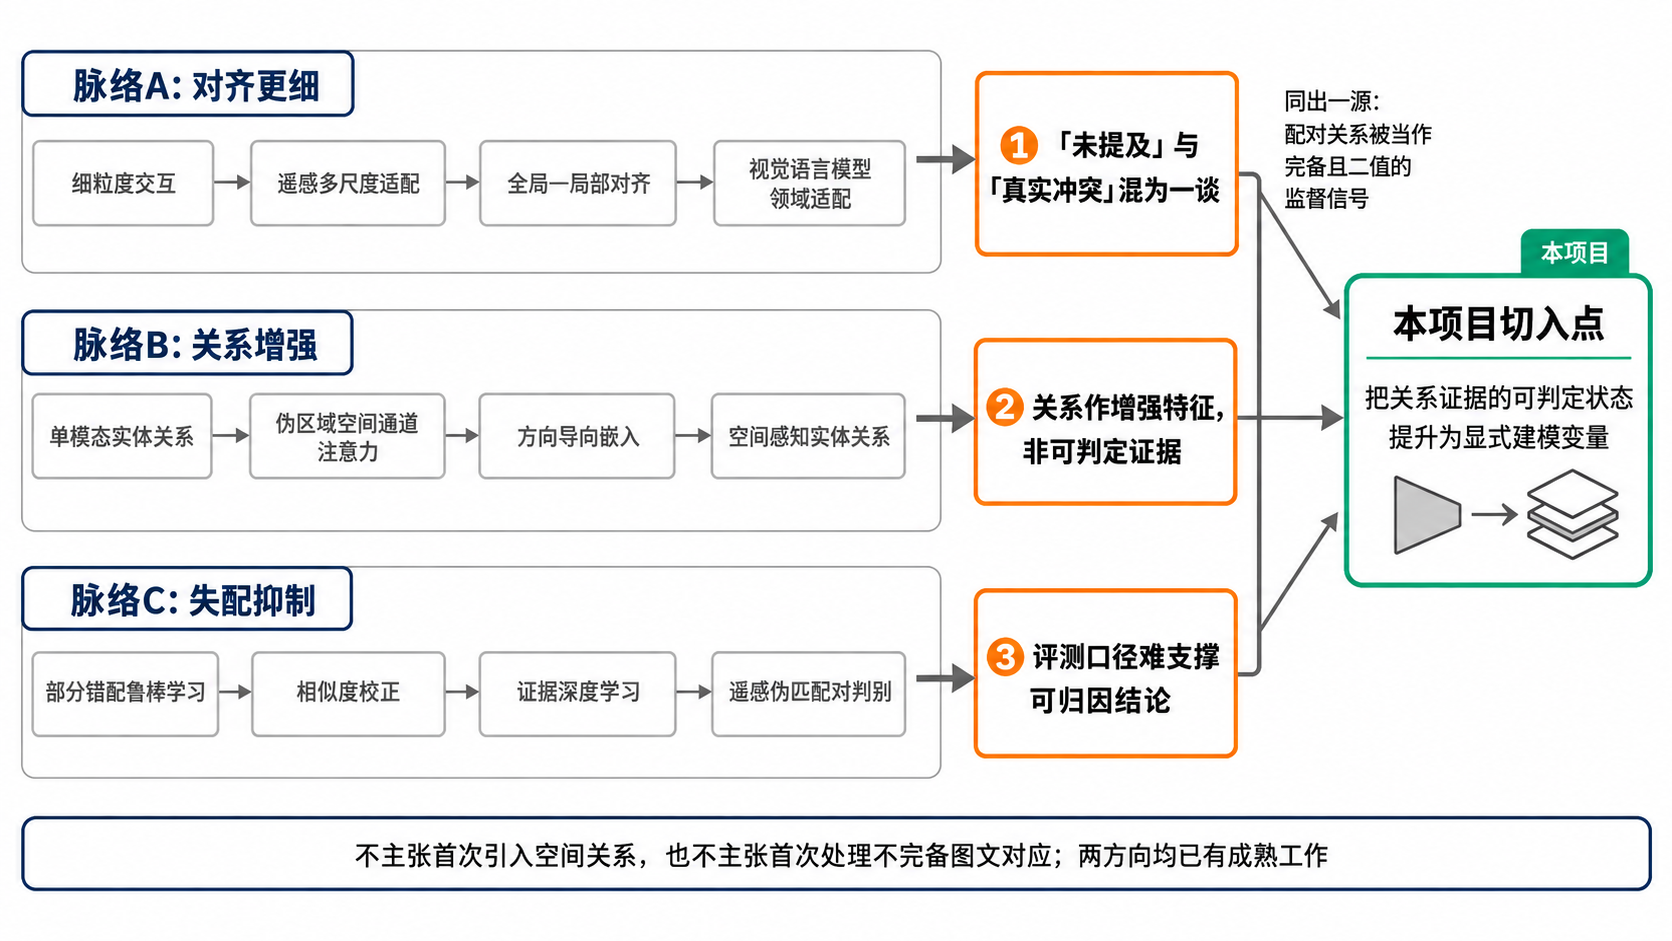
\includegraphics[width=\linewidth]{figures/F03_研究现状与切入点-v2.png}
    \caption{研究现状与本项目切入点。关系增强与失配处理已有研究基础，本项目关注关系证据的可判定状态。}
    \label{fig:landscape}
\end{figure}


\subsubsection{现有研究的不足}

综合上述现状，可以归纳出三点尚未被正面处理的问题。三者看似分属数据、方法与评测，实则同出一源：把图文配对关系当作完备且二值的监督信号。

\begin{enumerate}
    \item \itemtitlefont{"未提及"与"真实冲突"在建模上被混为一谈。} 面向不匹配的方法按失配强度统一抑制或重加权，不区分成因\cite{hu2023rcl,han2023msc,yang2023bicro,zhang2024npc,feng2024tripartition,pmpguard2026}。但在遥感图文数据中，描述不完备是\textbf{结构性属性}而非标注错误：同一影像的多条描述本就覆盖不同地物\cite{lu2018rsicd,yuan2022amfmn}。把"文本没写到"与"文本写错了"同等对待，前者会被施加本不该有的负样本惩罚，后者所携带的关系判别信息则被稀释。

    \item \itemtitlefont{关系被用作增强特征，而非可判定的证据。} 已有引入实体与空间关系的工作以关系增强表示与对齐为目标\cite{zhang2023unimodal,shui2025esrn,wu2024scat,yang2024dove,mi2024knowledgeaware}，隐含假设是关系标注可得且可靠。但图像级描述并不提供实体框、关系图或空间拓扑真值，自动抽取的三元组属于弱监督或伪标注，难以直接充当可信的评测标签。"这条关系在影像中究竟能否被判定"这一问题，尚未被作为一等建模对象处理。

    \item \itemtitlefont{评测口径难以支撑可归因的结论。} 综述已指出跨论文数字因协议差异而难以统一比较\cite{rsitrreview2025}；同时，预训练数据与检索基准之间存在重叠\cite{liu2024remoteclip}，大规模数据集又普遍依赖自动生成描述\cite{rsitrreview2025,zhang2024rs5m}。在缺少近重复去重与分层报告的情况下，性能提升可能来自骨干容量、训练预算或数据泄漏，而非所声称的机制。
\end{enumerate}

\subsubsection{关键科学问题与研究切入点}

\subsubsubsection{关键科学问题}

本项目拟解决的关键科学问题是：

\begin{quote}
\textbf{在遥感图文数据中文本描述对影像内容的覆盖天然不完备的条件下，如何在跨模态匹配中区分"描述未覆盖"与"实际关系冲突"，使有证据的地理实体关系参与约束、而不可判定的关系不被当作监督信号？}
\end{quote}

围绕这一问题，形成三个相互支撑的子问题：（1）\textbf{表示层}，如何构建带证据与置信度的实体—关系记录，使"已支持、明确冲突、未知"三态可判定、可人工复核；（2）\textbf{学习层}，三态信息以何种方式进入对齐或重排序目标，才能在不牺牲标准配对召回的前提下降低关系冲突导致的误匹配；（3）\textbf{验证层}，如何构造评测协议，使性能变化可归因于关系建模本身，而非骨干容量、训练预算或数据泄漏。

这里有必要交代它为什么是科学问题。工程问题的特征是目标明确、只需在既定评价函数下寻优；本问题触及的却是\textbf{评价函数本身的合法性}——对比学习框架中"未配对即为负例"的假设，在描述天然不完备的数据上并不总是成立，于是"优化得更好"与"优化得更对"可能指向不同方向。要回答它，必须先定义关系证据的可判定状态这一此前不存在的变量，再确定该变量以何种方式约束监督信号，最后建立能把效果归因到该变量的验证方式。这三步都不是参数调优或工程实现所能替代的。此外，本问题具有可证伪结构：如果错误归因表明描述不完备并非重要误差来源，或三态区分相对二值处理没有可复现的差异，则该问题的科学价值即被否定。可被否定，正是它作为科学问题的标志。

\subsubsubsection{研究思路与拟检验的假说}

本项目的切入点是把"关系证据的可判定状态"从隐含前提提升为显式建模变量。基本思路是：利用同一影像多条描述之间的\textbf{覆盖差异}作为天然信号，构建关系证据的三态表示；在已有视觉语言编码器基础上，仅对有证据的关系施加约束、对未知关系屏蔽监督；再通过标准检索与关系挑战的分层评测检验其效果。

据此提出三条可证伪假说。\textbf{H1（现象存在性）}：在公开基准的检索错误中，存在可稳定识别的一类——文本与影像在关系上并不冲突，仅因描述未覆盖部分地物而被判为低相似度。\textbf{H2（机制判断）}：把"未提及"当作负例监督会在关系敏感样本上引入系统性偏差；仅对有证据的关系施加约束、对未知关系屏蔽监督，可在保持标准 mR 不下降的前提下降低关系冲突误匹配。\textbf{H3（可归因性）}：上述改进不能由骨干容量或训练预算解释。

三条假说均设定了明确的证伪条件。若第一年的错误归因表明该类错误占比低于预设阈值\textbf{【暂定 10\%】}，或无法与"细粒度语义不足""同类场景近似"等既有成因稳定区分，则 H1 被证伪，本项目将据此调整研究内容一的定位乃至题目，而不会通过反向挑选样本维持原有结论。

\subsubsubsection{预期贡献}

本项目预期形成三方面贡献：在\textbf{问题层面}，澄清跨模态匹配中"未提及即不存在"这一默认前提在遥感场景下的不成立之处，给出可操作的三态区分；在\textbf{方法层面}，提出仅约束可核验关系、屏蔽未知态的匹配方式，并通过严格对照厘清其与"未知作负例""硬关系约束"两种处理的效果边界；在\textbf{评测层面}，建立标准检索与关系挑战分层报告、含近重复去重与等预算对照的验证协议，使关系建模的作用可被独立检验。

需要说明的是，本项目\textbf{不主张}首次引入空间关系或首次处理不完备图文对应——如前所述，这两个方向均已有成熟工作。本项目主张的是对关系证据状态的显式区分及其在监督信号构造中的作用，这是一个方法层面的问题重述与验证设计。
